\documentclass{beamer}
\usepackage{graphicx}
\usepackage{amssymb,amsfonts,amsmath}
% \usepackage{tikz,tkz-euclide}
% \usepackage{subfigure}
% \usepackage{parskip}
% \usetikzlibrary{arrows.meta}
% \usetikzlibrary{calc,patterns}
\usefonttheme[onlymath]{serif}
\usepackage{multimedia}
% \usetheme{Berlin}
\title{Weekly Report}
\author{WU Zihan}
\begin{document}
\maketitle
\begin{frame}
    \frametitle{Outline}
    \tableofcontents
\end{frame}

\section{Dancing}
\begin{frame}
    \frametitle{Dancing Dataset}
    % columns
    \begin{columns}
        \column{0.5\textwidth}
        % \movie[width=8cm,height=4.5cm,showcontrols=true,poster]{}{/Users/zihanwu/Public/codes/PhantomDanceDataset/Recordings/Movie_001.mp4}
        % figure dataset.jpg
        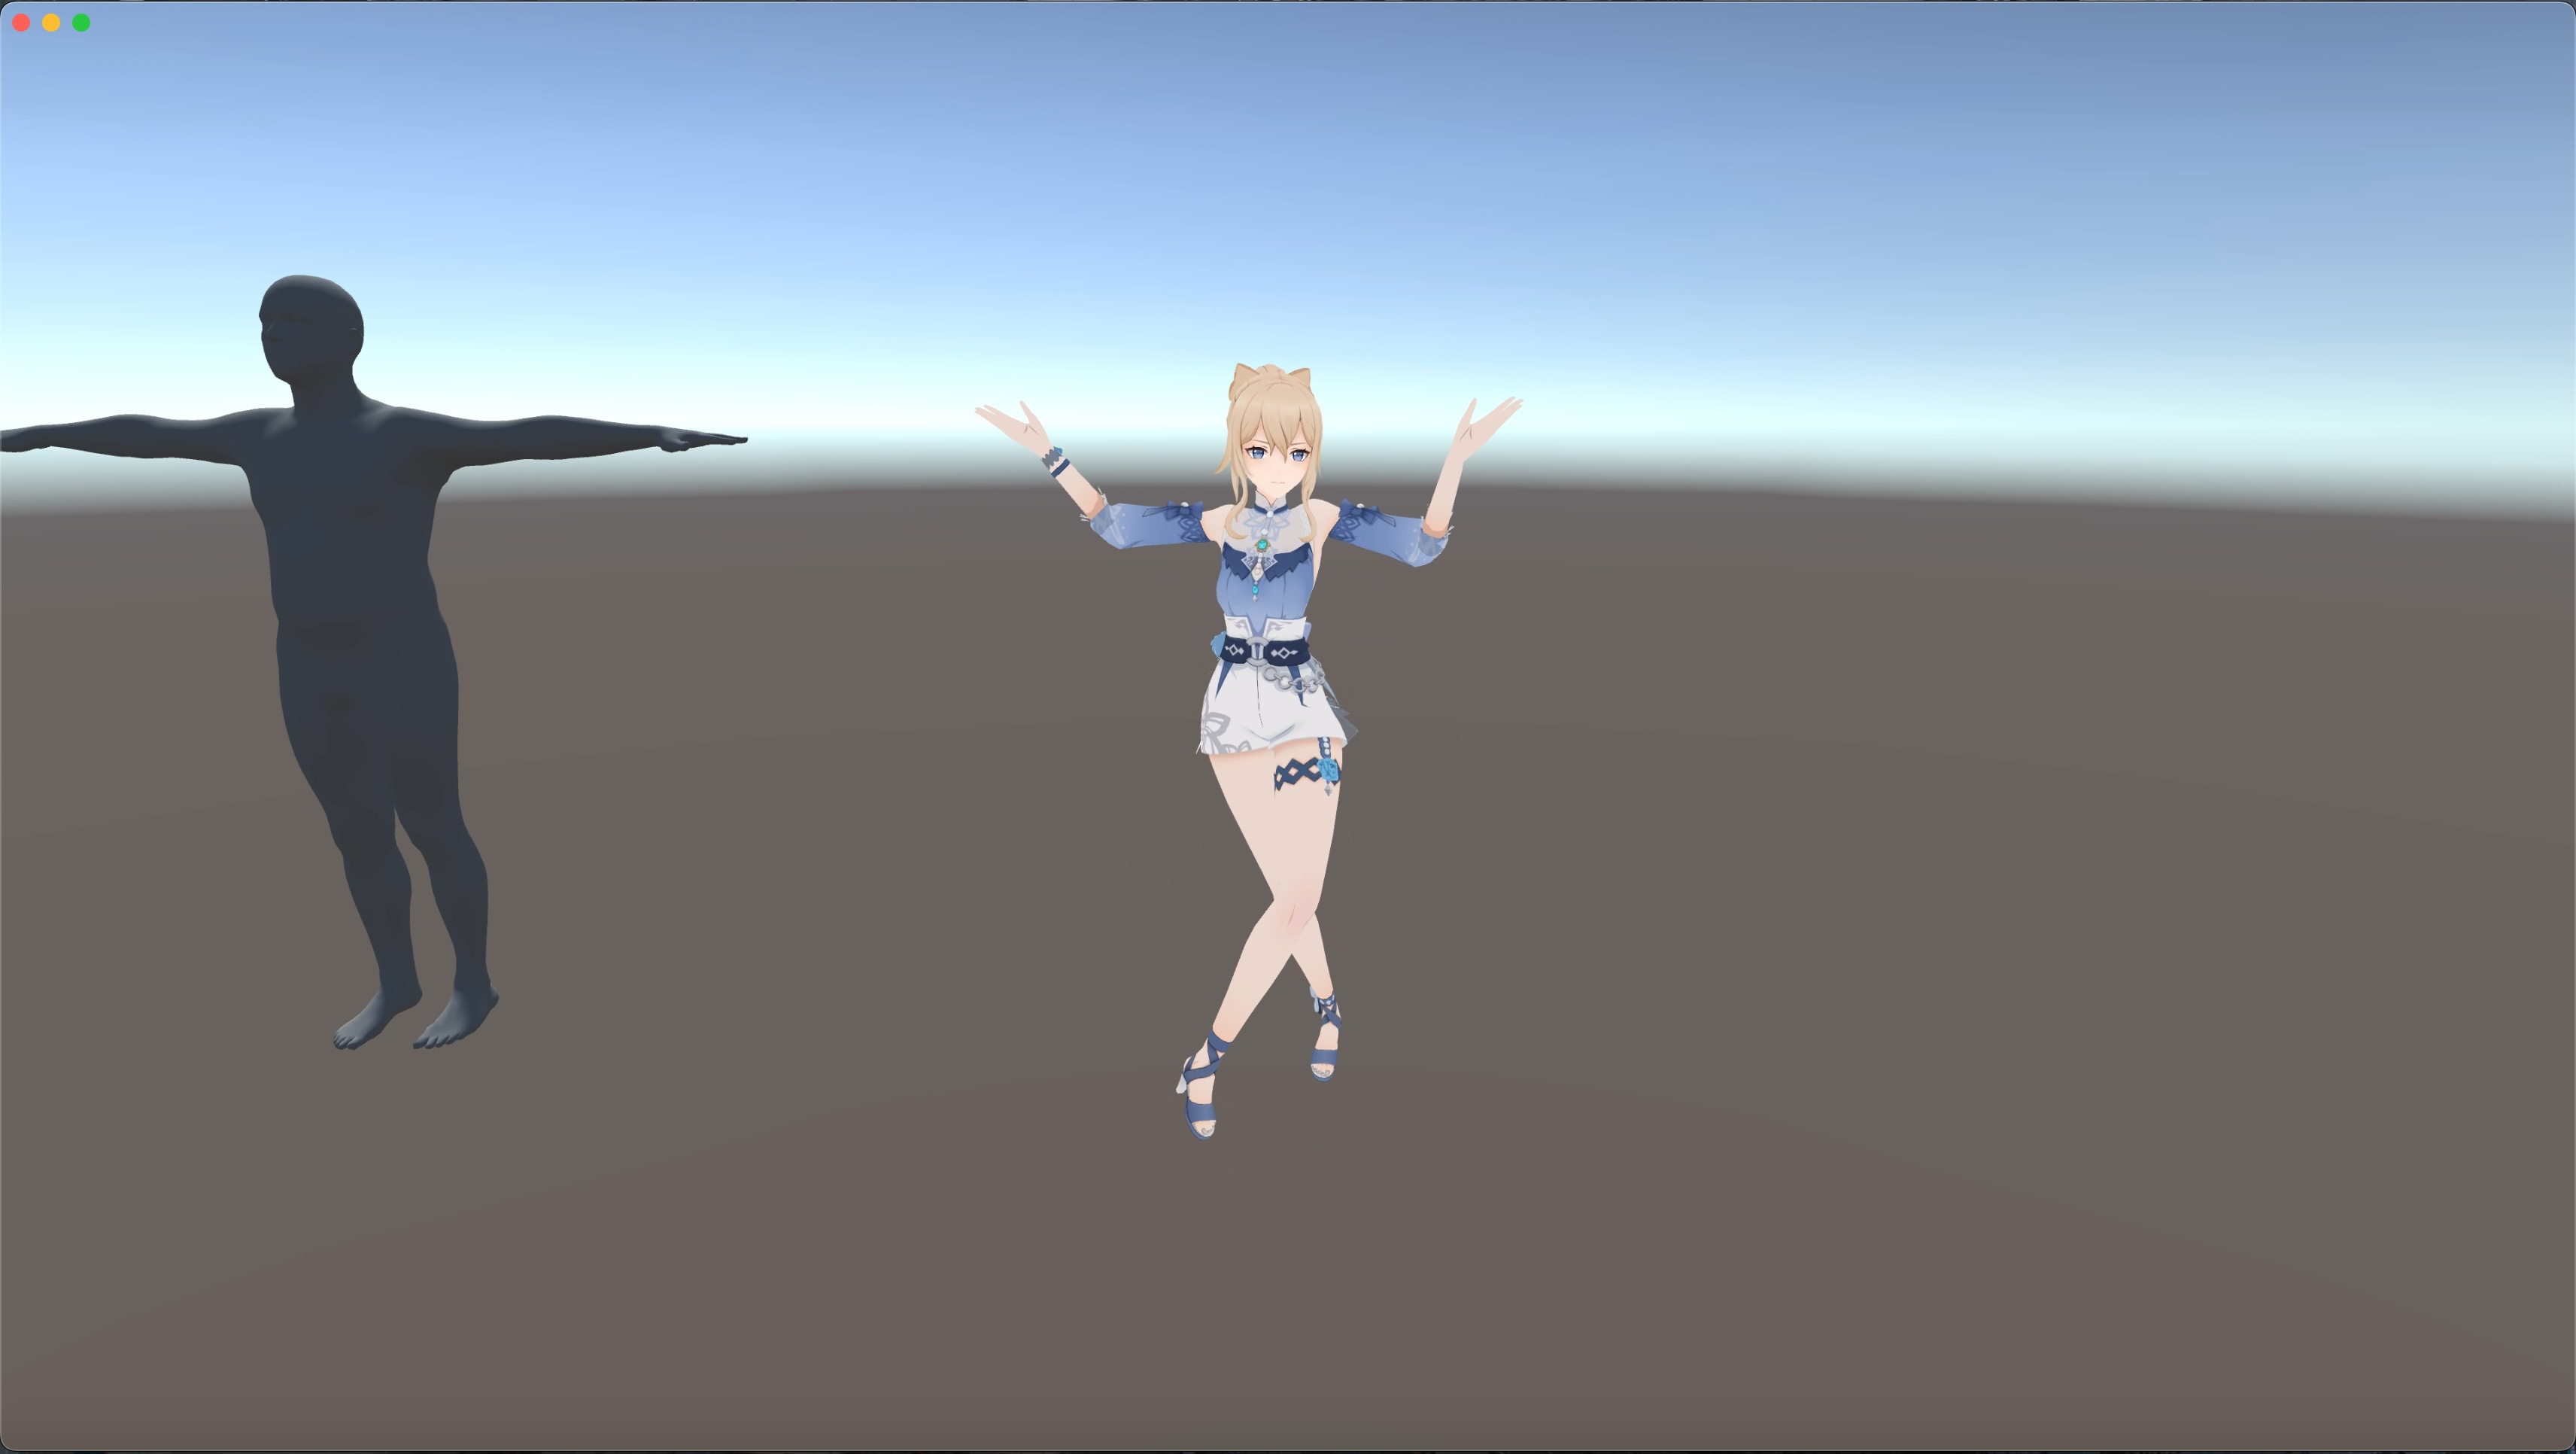
\includegraphics[width=\textwidth]{dataset.jpg}
        \column{0.5\textwidth}
        \begin{itemize}
            \item Conclusion: not so suitable for our task
            \item Reason: the dataset is complicated and the information is rich, resulting high-rank for feature matrix
            \item Pure quaternion / quaternion + mirror / Iisignature / Mirrored Iisignature are tried as features
        \end{itemize}
    \end{columns}
\end{frame}

\section{NLP Dataset}
\begin{frame}
    \frametitle{NLP Dataset}
    % columns
    \begin{columns}
        \column{0.5\textwidth}
        % time.jpg
        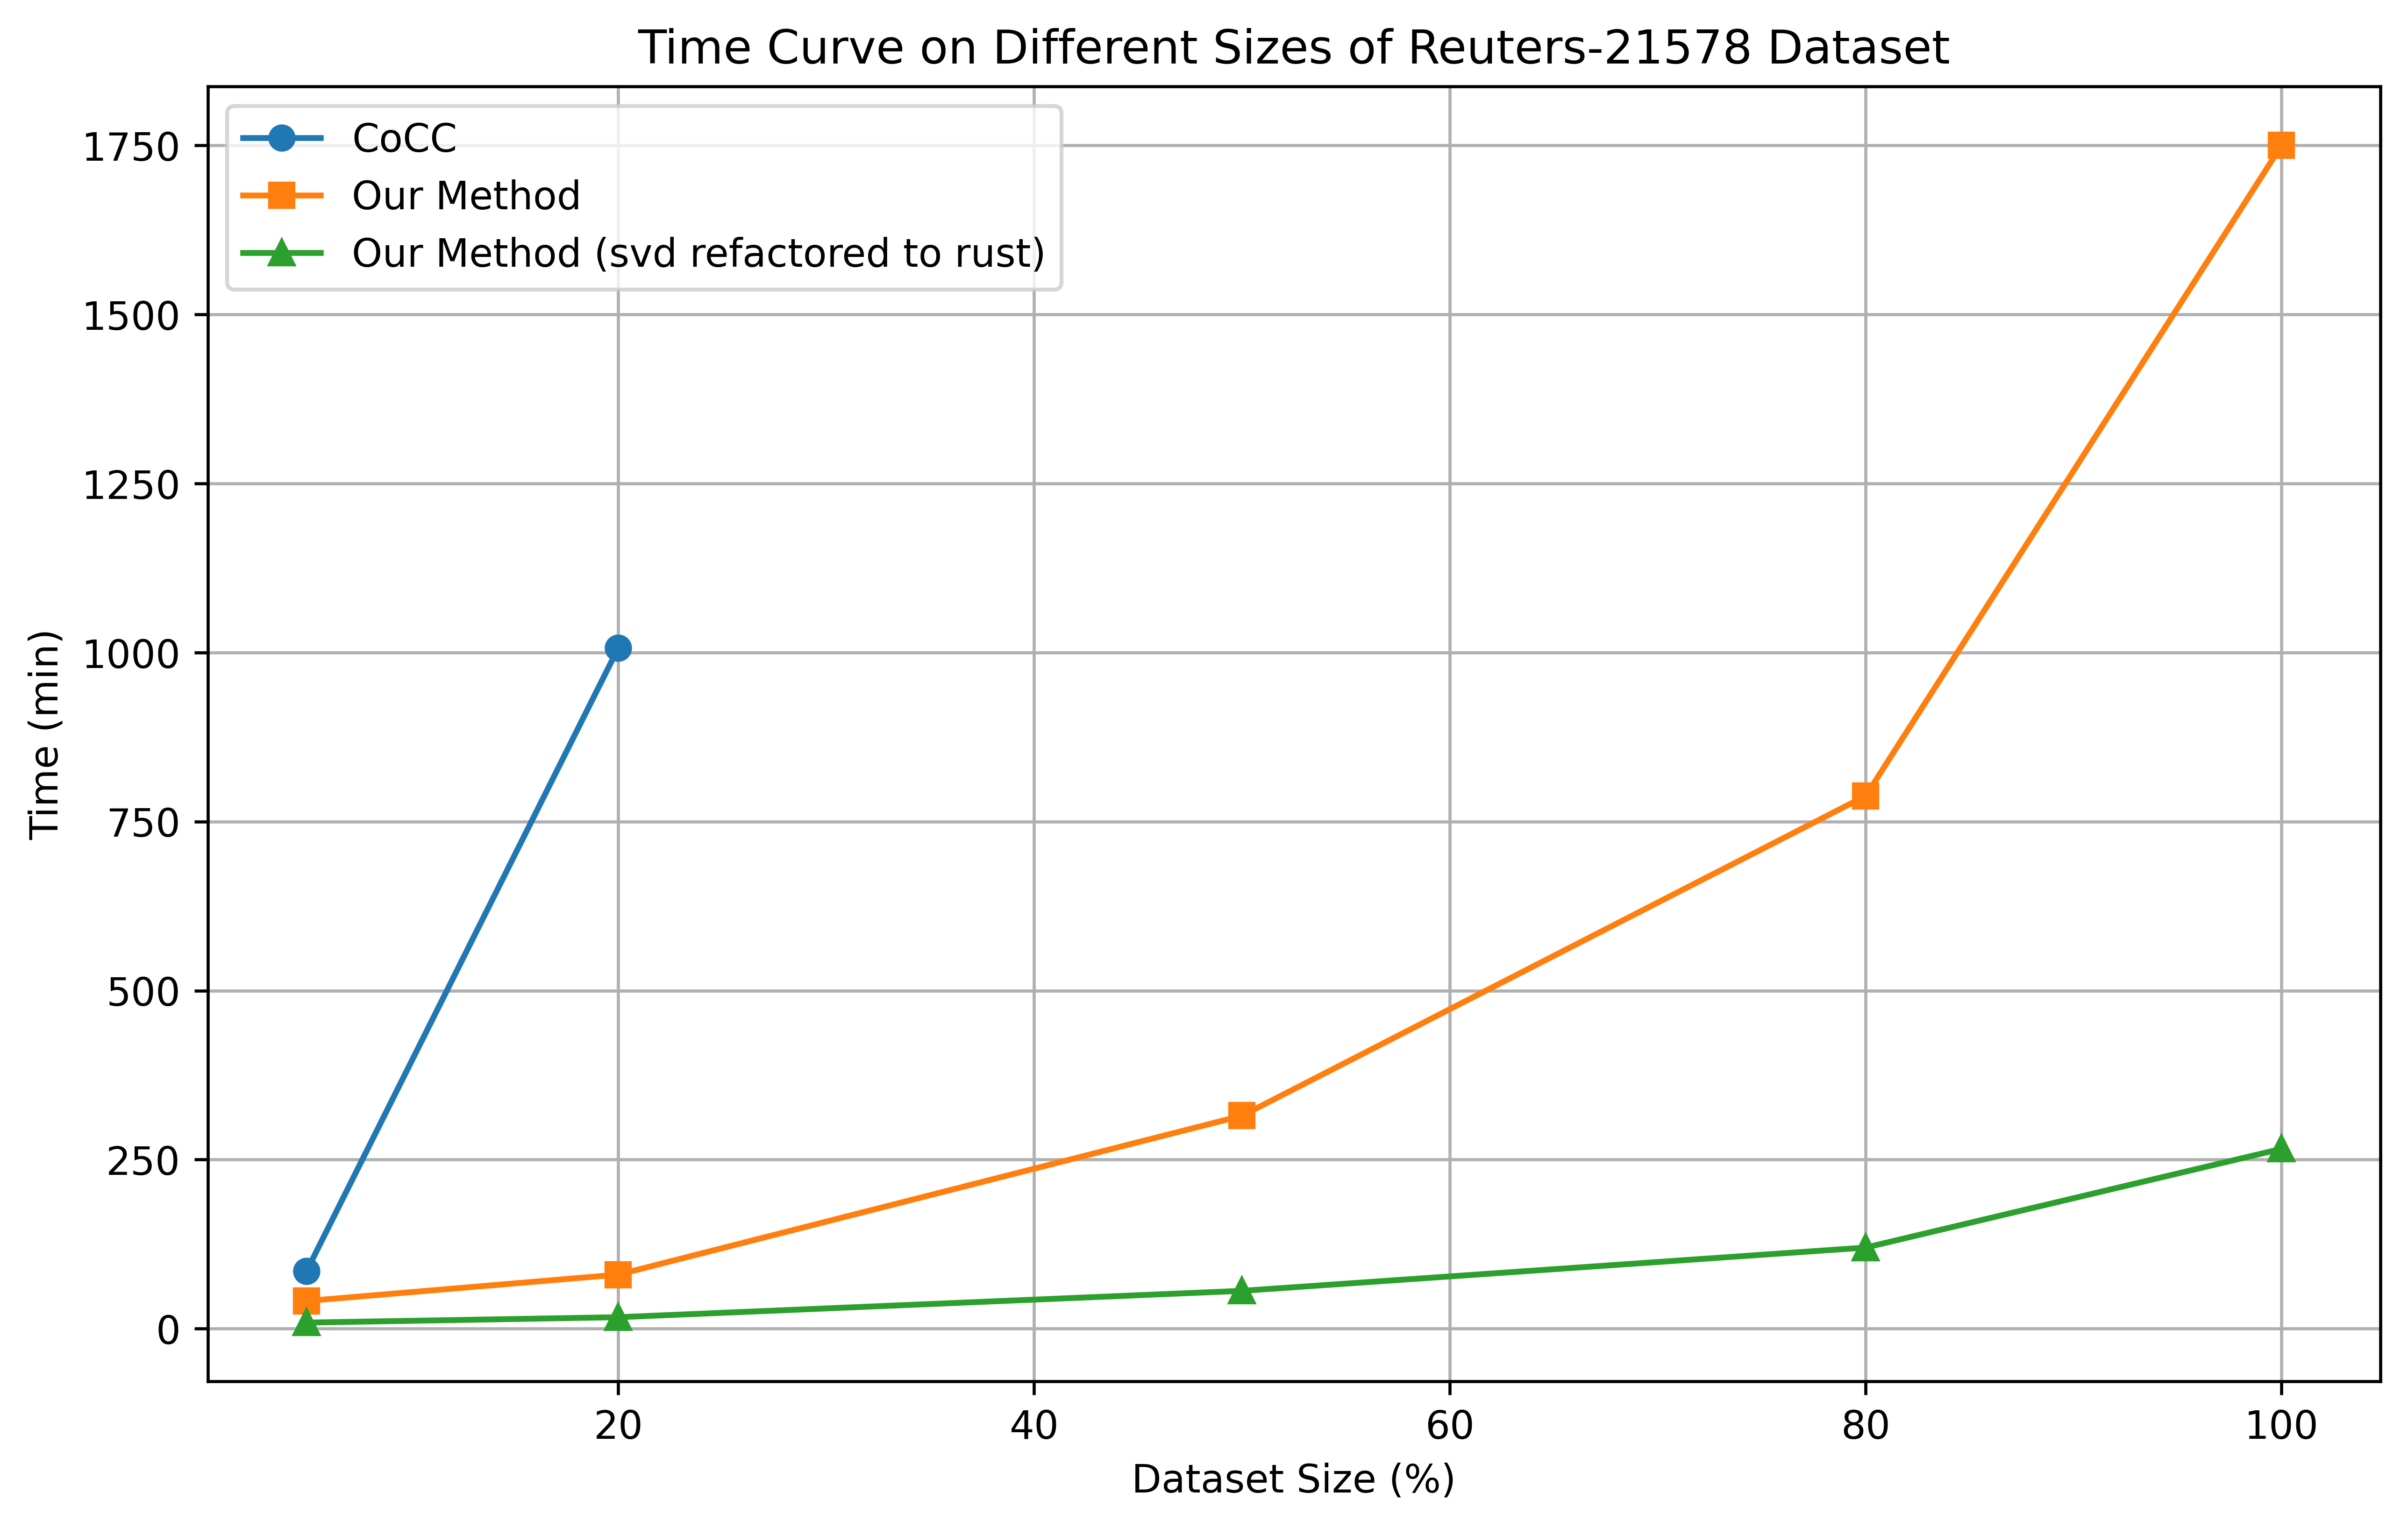
\includegraphics[width=1.1\textwidth]{time_curve.png}
        \column{0.5\textwidth}
        \begin{itemize}
            \item Reuters-21578
            \item 21,578 documents, 135 topics
            \item The memory consumption prevents us from using python to calculate on the bigger dataset (Trying MovieLens Dataset)
            \item Using rust to refactor the calculation part on the submatrix
        \end{itemize}
    \end{columns}
\end{frame}


\end{document}